\newcommand{\ASKA}{$\text{ASK}^0$}
\newcommand{\ASKS}{$\text{ASK}^*$}

\chapter{Literature Review}

In this chapter it will be discussed some basic concepts to better understand this thesis work. First, it will be introduced the concept of  recommender systems (RS) and their importance to today's online business. Second, the metric used to evaluate the performance of the RS algorithm: lift. After that, a general discussion of clustering will be presented followed by one technique to visualize the clusters of a dataset: Principal Component Analysis.


\section{Recommender systems}

A RS is a software which its main purpose, as the name suggests, is to give suggestions \cite{ricci2011introduction} or recommendations to a user based on information about the user itself or the context of the items to recommend. They are classified as part of information filtering systems \cite{RecommendersystemWikipedia}. So, another way to interpret the recommendations is to think as a result of a filter applied on a search space, where only the most relevant information is given back to the user. It is important to emphasize that usually the search space on the RSs today are enormous. For example, there are more than 400 million products on Amazon US available \cite{amazon-number-of-products-2015}. Meaning that, in terms of time, it is unreasonable for a human to search one by one. Hence, the importance of these type of system on the applications today.

\subsection{Types of Recommender Systems}

There are three main types: the ones based on \textbf{collaborative filtering}, the ones on \textbf{content-based filtering}, and \textbf{hybrid}. 

The first one is \textbf{collaborative filtering}, where the recommendations come mainly from information generated by the user and its interaction with the items. For instance, one type of logic is the \textbf{user-based}, where a item is recommended to the user based on what other similar users like, more known as \textit{people like you, also like X}. Another logic is the \textbf{item-based} one, where the RS acts based on the similarity between items, also known as \textit{if you like X you may like X}. Figure \ref{fig:colab-filt-user-user} shows an example of user-based collaborative filtering, where the RS wants to predict what is the preference on headphones of user E. Based on users B and C (they voted similarly to E), we can see that, probably its an \textit{dislike}.

\begin{figure}[h]
   \centering
   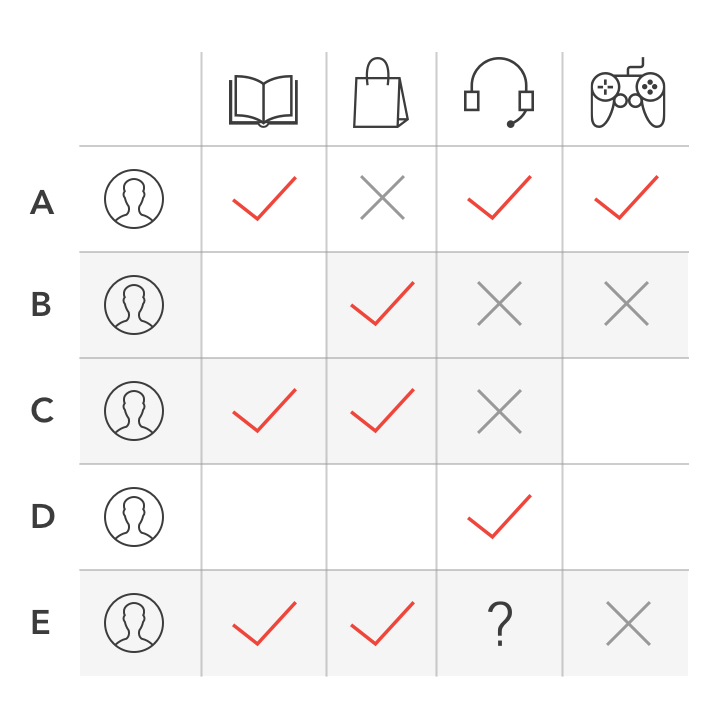
\includegraphics[width=6cm]{fig/ch2-colab-filt-user-user.jpg}
   \caption{User-based logic on collaborative filtering. Source: \cite{delawareai}}
   \label{fig:colab-filt-user-user}
\end{figure}

The second one is \textbf{content-based filtering}, where the recommendations are based on the features of the items and more importantly: an \textbf{user profile}. The system needs an input from the user, be it interactively like in a sequential manner or historical data, or in a batch where the user gives a lot information about itself in one shot. Having the profile, the RS can cross this information with the features of the items to look for items that are similar to the user's profile. It can remember the item-based logic from collaborative filtering, but here we have added the information of the user. One example that illustrate content-based, is an article reader service. Imagine when one sign up to the service, it will ask a lot of question to the new user: "What type of articles you prefer: Sports, Politics, Health?", "What kind of Sports do you like: Soccer, Volleyball, Baseball...?". These questions build up a profile to new user and it will be refined as the users utilizes the service. Therefore, if our hypothetical new user answers "Sports" and "Soccer" to the previous questions, the article service will start recommending articles of soccer. But if this new user only thumbs up Brazilian Soccer articles, the RS will learn that and narrow down the recommendations to Brazilian soccer.

Finally, there is the \textbf{hybrid} type, where the Recommendation System is based on a mixture of both previous types. Combining them can improve the recommendations and at the same time deal with their constraints. Collaborative filtering has the problem of \textbf{cold start}, whenever a new item or user is added, it has no attributes. So it will take some time until its attributes are filled up. This problem leads to another one which is the \textbf{sparsity} on the matrix of attributes. Meaning that, there are a lot of missing values. Content-based filtering can supply this data to the RS. And combining with the accuracy of collaborative filtering the system can achieve very personalized recommendations.


\subsection{Benefits on business}

The RSs are present on a myriad of online services today, bringing great value to them. Streaming platforms of music and videos have RSs on their business to increase user retention and engagement such as: 75\% of what people watch on Netflix come from recommendations \cite{HowretailerscankeepupwithconsumersMcKinsey} or that 70\% of people's time spent on YouTube comes from the recommendation of "the Algorithm" \cite{CES2018YouTubesAIrecommendationsdrive70percentofviewingCNET}. Social medias and reading platforms apply these same concepts on their "feed" for the same reasons of streaming platforms, user retention and engagement. E-commerce, on the other hand, want to increase their revenue by recommending similar products, or products that the "same type of customer purchased" when a potential customer is navigating on their online shop. Amazon is a great example of this: 35\% of the purchases on their online shopping come from recommendations \cite{HowretailerscankeepupwithconsumersMcKinsey}. There is even the use of RSs on online dating services \cite{brozovsky2007recommender}, where the RS improve the experience of the user in the search of potential partner while at the same time increasing the monetization of the service. All of these business make use of this technology, but there is also the ones that gave back to the research of RS.

Netflix is one of the companies that are references on this type of system. They have a variety of algorithms on their RS. And due to the high user base, they can test their results using A/B testing and feedback from the users \cite{gomez2016netflix}. IN 2006 they launched a competition, called the Netflix Prize, where the objective was to improve the accuracy of the recommendations by 10\%. The winner would win US\$ 1.000.000. There were more than 2.000 teams and more than 40.000 submissions on their platform. The Netflix prize was an important event to the RSs in general because it increased the awareness of this technology, and its importance to business, worldwide. 

\subsection{Evaluation}
\label{ch:evaluation}

There are several ways to evaluate the performance of a recommender system: normalized Discounted Cumulative Gain (nDCG) \cite{jarvelin2002cumulated}, Precision \cite{Precision-rs-metric}, Recall \cite{cremonesi2010performance} when "looking" to the RS with a ranking perspective; Mean Absolute Error (MAE) \cite{breese1998empirical} and Root Mean Squared Error (RMSE) \cite{bennett2007netflix} when "looking" to the RS with a rating perspective; A/B testing when you have a high client base that guarantee statistical relevance and others \cite{parra2013recommender}. To evaluate the Neoway's recommender system we chose the Lift.

Lift is a ratio between probabilities. The probability of selecting one of the target population after the RS sorting versus the random  chance (before the RS sorting). The lift, is usually expressed in terms of quantiles. \cite{LiftAnalysisADataScientistsSecretWeapon}.
\begin{equation}
% TODO fix the non space on the formula
	lift = \frac{RS sorting prob}{random chance}
\end{equation}

To illustrate further, let us use an example of a box with colored balls. Imagine that there is a rectangular box where its height and depth allows only a single ball to fit, but its width allows up to 100 balls. There are two types of balls: the \textbf{red} ones that represent our \textbf{target population} and the blue ones. 90 of the 100 balls are blue and the remaining 10 are red. Moreover, this box is divided into sectors where each sector is a decile, meaning that there are 10 sectors, each one with 10 balls. The sectors, also, have a priority, they from left to right. The Figure \ref{fig:rec-box} shows hows this box looks like.

\begin{figure}[h]
   \centering
   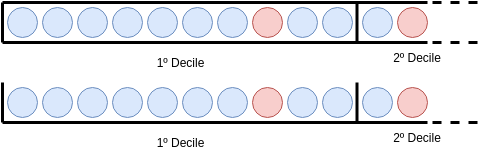
\includegraphics[width=\linewidth]{fig/ch2-rec-box.png}
   \caption{Rectangular box. Upper view (above), Front view (below).  Source: Author}
   \label{fig:rec-box}
\end{figure}

Without seeing inside the box, the probability of retrieving a red ball is 10 out of 100, or \textbf{10\%}. This is our \textbf{random chance} and it is the same probability for each decile. Now lets consider that someone reordered the balls (representing the RS), trying to place the red ones on first deciles. The Figure \ref{fig:rec-box-ordering} shows the box before and after the reordering.

\begin{figure}[h]
   \centering
   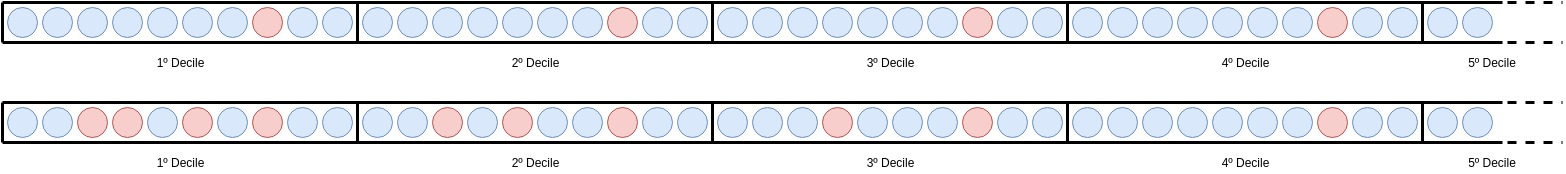
\includegraphics[width=\linewidth]{fig/ch2-rec-box-ordering.jpg}
   \caption{Reordering of the balls. Before (above) and after (below). Source: Author}
   \label{fig:rec-box-ordering}
\end{figure}

After the reordering, we recalculate the probabilities of retrieving a red ball for each decile. We can see on Figure \ref{fig:rec-box-ordering}, that there are 4 red balls on the first decile, 3 on the second, 2 on the third and 1 on the fourth. With this information we have the following probabilities, respectively: 40\%, 30\%, 20\%, 10\% and 0\% to the remaining deciles. Now the lift for the deciles can be calculated, for the first one is:
\begin{equation}
	lift_{1\textsuperscript{o} decile} = \frac{0.4}{0.1} = 4
\end{equation}

Using the same approach, we calculate the lift for the others deciles, respectively: 3, 2, 1, and 0 to the remaining ones. Figure \ref{fig:lift-plot} shows a plot of the values of the lift for each decile.

\begin{figure}[h]
   \centering
   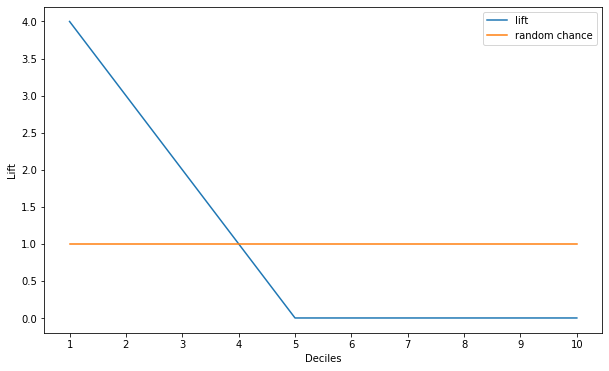
\includegraphics[width=9cm]{fig/ch2-lift-plot.png}
   \caption{Lift plot for the reordered box with the random chance. Source: Author}
   \label{fig:lift-plot}
\end{figure}

We can see that it is more likely to pick a red ball on the firsts sectors of our box (deciles) than the last ones. Actually, there is a zero probability to get a red ball after the fourth decile. And this is the expected behavior, since in an information retrieval system (IRS), we want all the relevant information on the top (in our case: on the left). Hence, only the first N-quantiles (in our case: N = 10) are considered and the rest is discarded. The designer of the system should decide how many quantiles are included and it also depends on how much information is retrieved and how much is processed by the user.

With this example, another way to interpret the lift is:  how many times better than the random chance is to get relevant information in the first N-quantiles ordered by an IRS. On the recommendations context the information is an item recommended and the IRS is the recommender system.

\section{Clustering}

% what % why
Cluster Analysis is a unsupervised learning technique where its objective is to find a finite and discrete set of "hidden" structure on a dataset \cite{xu2008clustering}. These structures or patterns can help better understand data or serve as preprocessing step for algorithms. Clustering, also, can be a way to represent large amounts of information which is equivalent to compressing data. 

% where
This technique is applied in several areas \cite{sabine2001cluster}. For instance, in Engineering and Computer Science, clustering is used in speech recognition, information compression, noise removal; In biology, the applications are: genetics, taxonomy, microbiology and others; It is also used in Astronomy and Geography on classification of galaxies, planets for the former and classification of regions, areas, vegetation and land for the latter.

% how
There are various approaches used to cluster a data set \cite{wikipedia_cluster_analysis}. The \textbf{Connectivity based} method looks for the closeness of two objects, meaning that it forms the clusters based on their distance which can be computed with different ways like the complete (maximum distances) or simple (minimum distance) linkage methods. The \underline{Hierarchical Clustering} is an example of algorithm that uses this approach; On \textbf{Centroid-based} clustering the data is represent by a vector of centroids - we can think of them like center of mass - one for each cluster. The \underline{KMeans} algorithm (and its variations), uses this approach. The \textbf{Distribution-based} approach focus on the statistics of the dataset. It groups together objects that have similar distributions. The algorithms to exemplify this are the \underline{Gaussian Mixture} and its \underline{Bayesian} variation. Another one is the \textbf{Density based} clustering where the data is grouped on the high density areas. Points that are to far away are considered outliers and do not go to any cluster. Common algorithms are the \underline{DBSCAN} and the \underline{OPTICS}.


% caveat
There is no single best algorithm on cluster analysis \cite{james2013introduction}. All of these presented, have pros and cons and are fit to different kind of problems. Some are suited to find the number of clusters but at the same time don't scale with a high volume of data (Hierarchical), others are fast and simple but they have to know the number clusters in advance (KMeans). Hence, its important to test different algorithms and its parameters to see if the analysis performs on a given problem.
% Didn't like this last sentence

\section{Principal Component Analysis}

% what
Principal Component Analysis, or PCA for short, is a orthogonal linear transformation \cite{wikipedia_pca} where you "break down" a dataset - that can have correlation between the features - into independent set of values called \textbf{Principal Components}. These components hold the how much variance the data have, or in practical terms, the amount of information. They are sorted in a descending fashion, where the first principal component (PC1) have the most variance and PC-N, have the least variance. N goes up to the number of features/variables or number of rows, the minimum between these two. 

%how
To understand how the PCA works in an intuitively way, the Figure \ref{fig:pca-steps} illustrate the steps of the PCA algorithm on a dataset with two variables.

\begin{figure}[h]
   \centering
   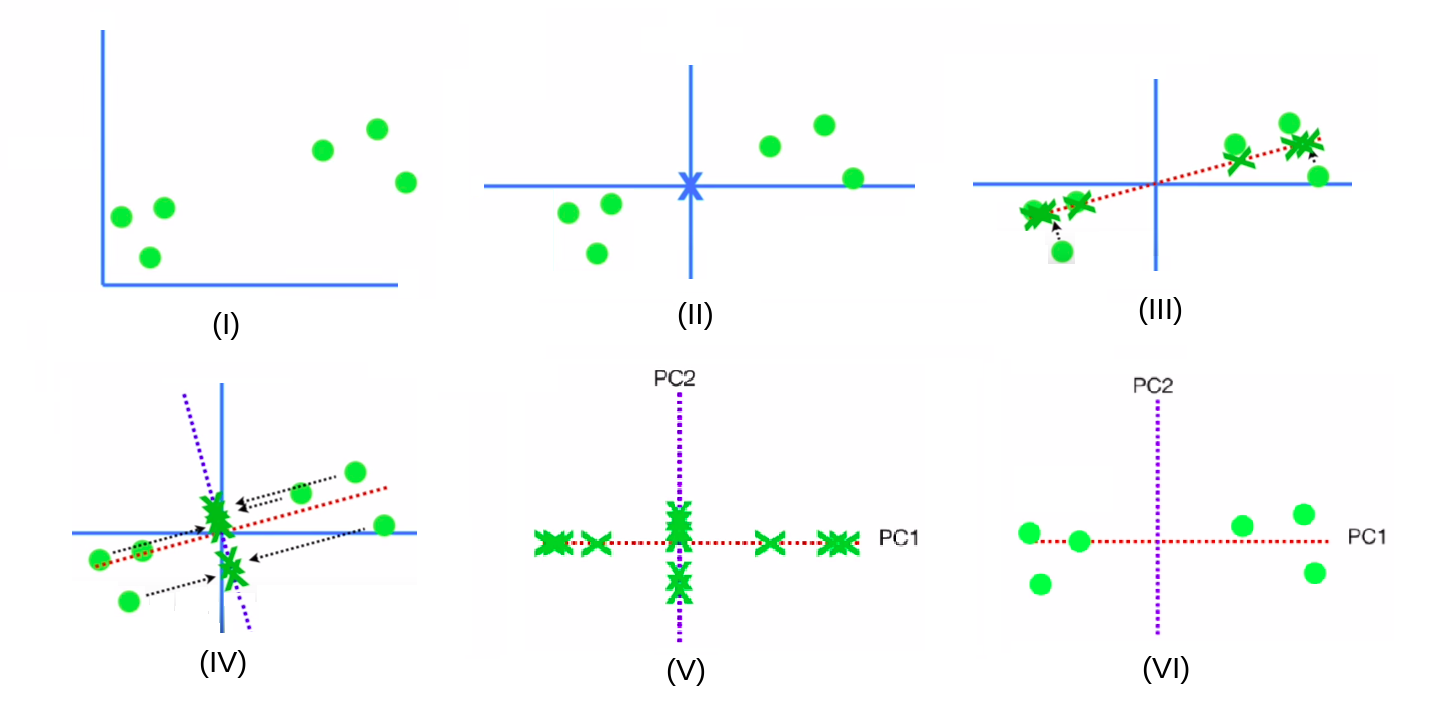
\includegraphics[width=\linewidth]{fig/ch2-pca-steps.png}
   \caption{Steps of PCA for two variables. Source: Adapted from \cite{pcastepsyoutube}.}
   \label{fig:pca-steps}
\end{figure}

From the original data (I) we calculate the mean point (center of mass), by getting the means of the x-axis and y-axis. Then we make this point our new origin (II). After that, a line that goes through the origin is fitted on the data on the direction of the highest variance (III). This direction is obtained by maximizing the sum of squared distances from the origin of each point's projection on the line(represented by the green Xs). The best fitted line is the Principal Component 1 (PC1). To find PC2, a line that is perpendicular to PC1 should be fitted on the data using the same approach to find the second-highest-variance direction. However, since this example there are only two variables, there is only one possible direction (IV). With PC1 and PC2 calculated, when can make them our new axis (V) and use the points' projections (V) to find where they go on the PCA plot (VI). For a dataset with more variables the process is the same: data is centered; each PC(N) line should point to the direction of N-highest variance and every PC(N+1) must be orthogonal to PC(N). The method explained in this example is also known as \textbf{Singular Value Decomposition} (SVD).

%why and where
PCA can be applied to any numerical dataset \cite{wold1987principal} (first it must be transformed or scaled). It can be a useful tool to analyse any multi-variable data. One use of this technique is the \textbf{PCA plot} which consists on getting the first two or three principal components (PCs) and plotting the transformed data. Since most of the variance (information) is on the first PCs, we can use them to look for patterns on the dataset with 2-D or 3-D plots. One of the patterns that can be found are clusters \cite{ding2004k}. 

Another use of PCA is on \textbf{dimensionality reduction}. Imagine that there is a dataset with more than 200 variables. Due to the curse of dimensionality \cite{Bellman:2010:DP:1893145} or even computing power a reduction on the number features is needed. If by applying PCA on this dataset we get, for instance, 99\% of the variance on the first 20 PCs, the remaining PCs can be discarded. In practice, we are getting a 90\% data reduction with only 1\% of the information lost.





